% Name: Reaction energy profile
% Description: The energy of an exothermic reaction along its reaction coordinate: reactants, the transition state, products, the activation energy, ΔH, and a lower path with a catalyst.
% Tags: reaction profile, activation energy, enthalpy, catalyst

\usetikzlibrary{arrows.meta}

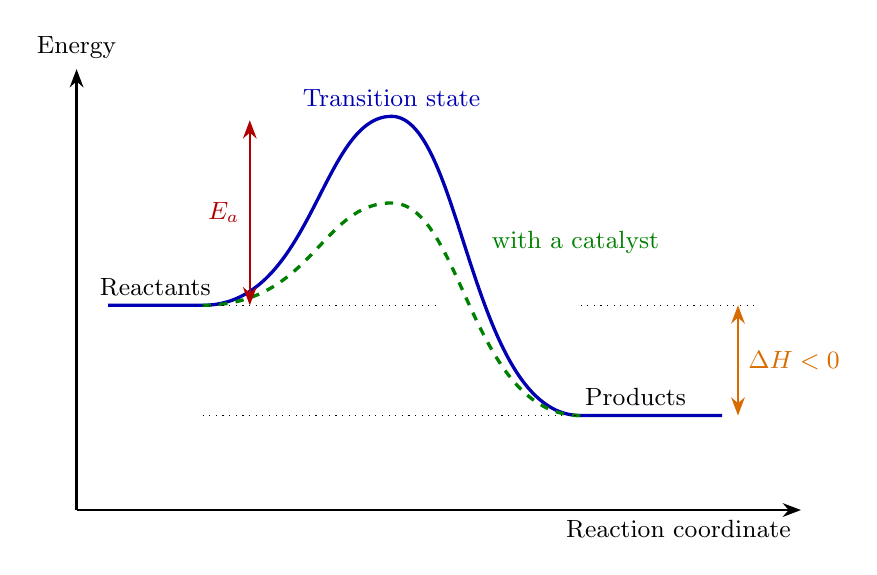
\begin{tikzpicture}[>={Stealth}, every node/.style={font=\small}]
  \draw[->, thick] (0,0) -- (9.2,0) node[below left] {Reaction coordinate};
  \draw[->, thick] (0,0) -- (0,5.6) node[above] {Energy};
  \draw[very thick, blue!70!black] (0.4,2.6) -- (1.6,2.6) .. controls (3,2.6) and (3.1,5) .. (4,5) .. controls (4.9,5) and (5,1.2) .. (6.4,1.2) -- (8.2,1.2);
  \draw[very thick, dashed, green!50!black] (1.6,2.6) .. controls (3,2.6) and (3.1,3.9) .. (4,3.9) .. controls (4.9,3.9) and (5,1.2) .. (6.4,1.2);
  \node[above] at (1,2.6) {Reactants};
  \node[above] at (7.1,1.2) {Products};
  \node[above, blue!70!black] at (4,5) {Transition state};
  \node[green!50!black, right] at (5.15,3.4) {with a catalyst};
  \draw[dotted] (1.6,2.6) -- (4.6,2.6);
  \draw[<->, thick, red!70!black] (2.2,2.6) -- node[left] {$E_a$} (2.2,4.95);
  \draw[dotted] (1.6,1.2) -- (6.4,1.2);
  \draw[dotted] (6.4,2.6) -- (8.6,2.6);
  \draw[<->, thick, orange!85!black] (8.4,1.2) -- (8.4,2.6) node[midway, right] {$\Delta H < 0$};
\end{tikzpicture}
